

% ==============================================================================
% ==============================================================================
\chapter*{Appendix A}  \addcontentsline{toc}{chapter}{Appendix A: Visualization} \label{vis}
% ==============================================================================
% ==============================================================================
\section*{Visualization}
The majority of the generated outputfiles of the provided simulation tools utilize
the CSV format.
This CSV format is supported by various available tools, such as
the free open source tools ParaView ~\cite{paraview}, or Gnuplot~\cite{gnuplot} and the commercial MATLAB~\cite{matlab} suite.

In the following an exemplary visualization approach based on ParaView (Version 3.98.0) is depicted.
The first step of processing a CSV file is to load it via the \texttt{Open File} dialog.
As the the CSV output files generated by a ViennaWD simulator offer the \texttt{*.csv} file extension,
ParaView applies the corresponding file-processer automatically.
Fig.~\ref{fig:para1}-\ref{fig:para7} show the required steps. Several Paraview state files, containing predefined filter sequences, are included with the WEMC simulator under \texttt{wigner\_ensemble\_monte\_carlo/plot\_scripts} 

\begin{figure}[!ht]
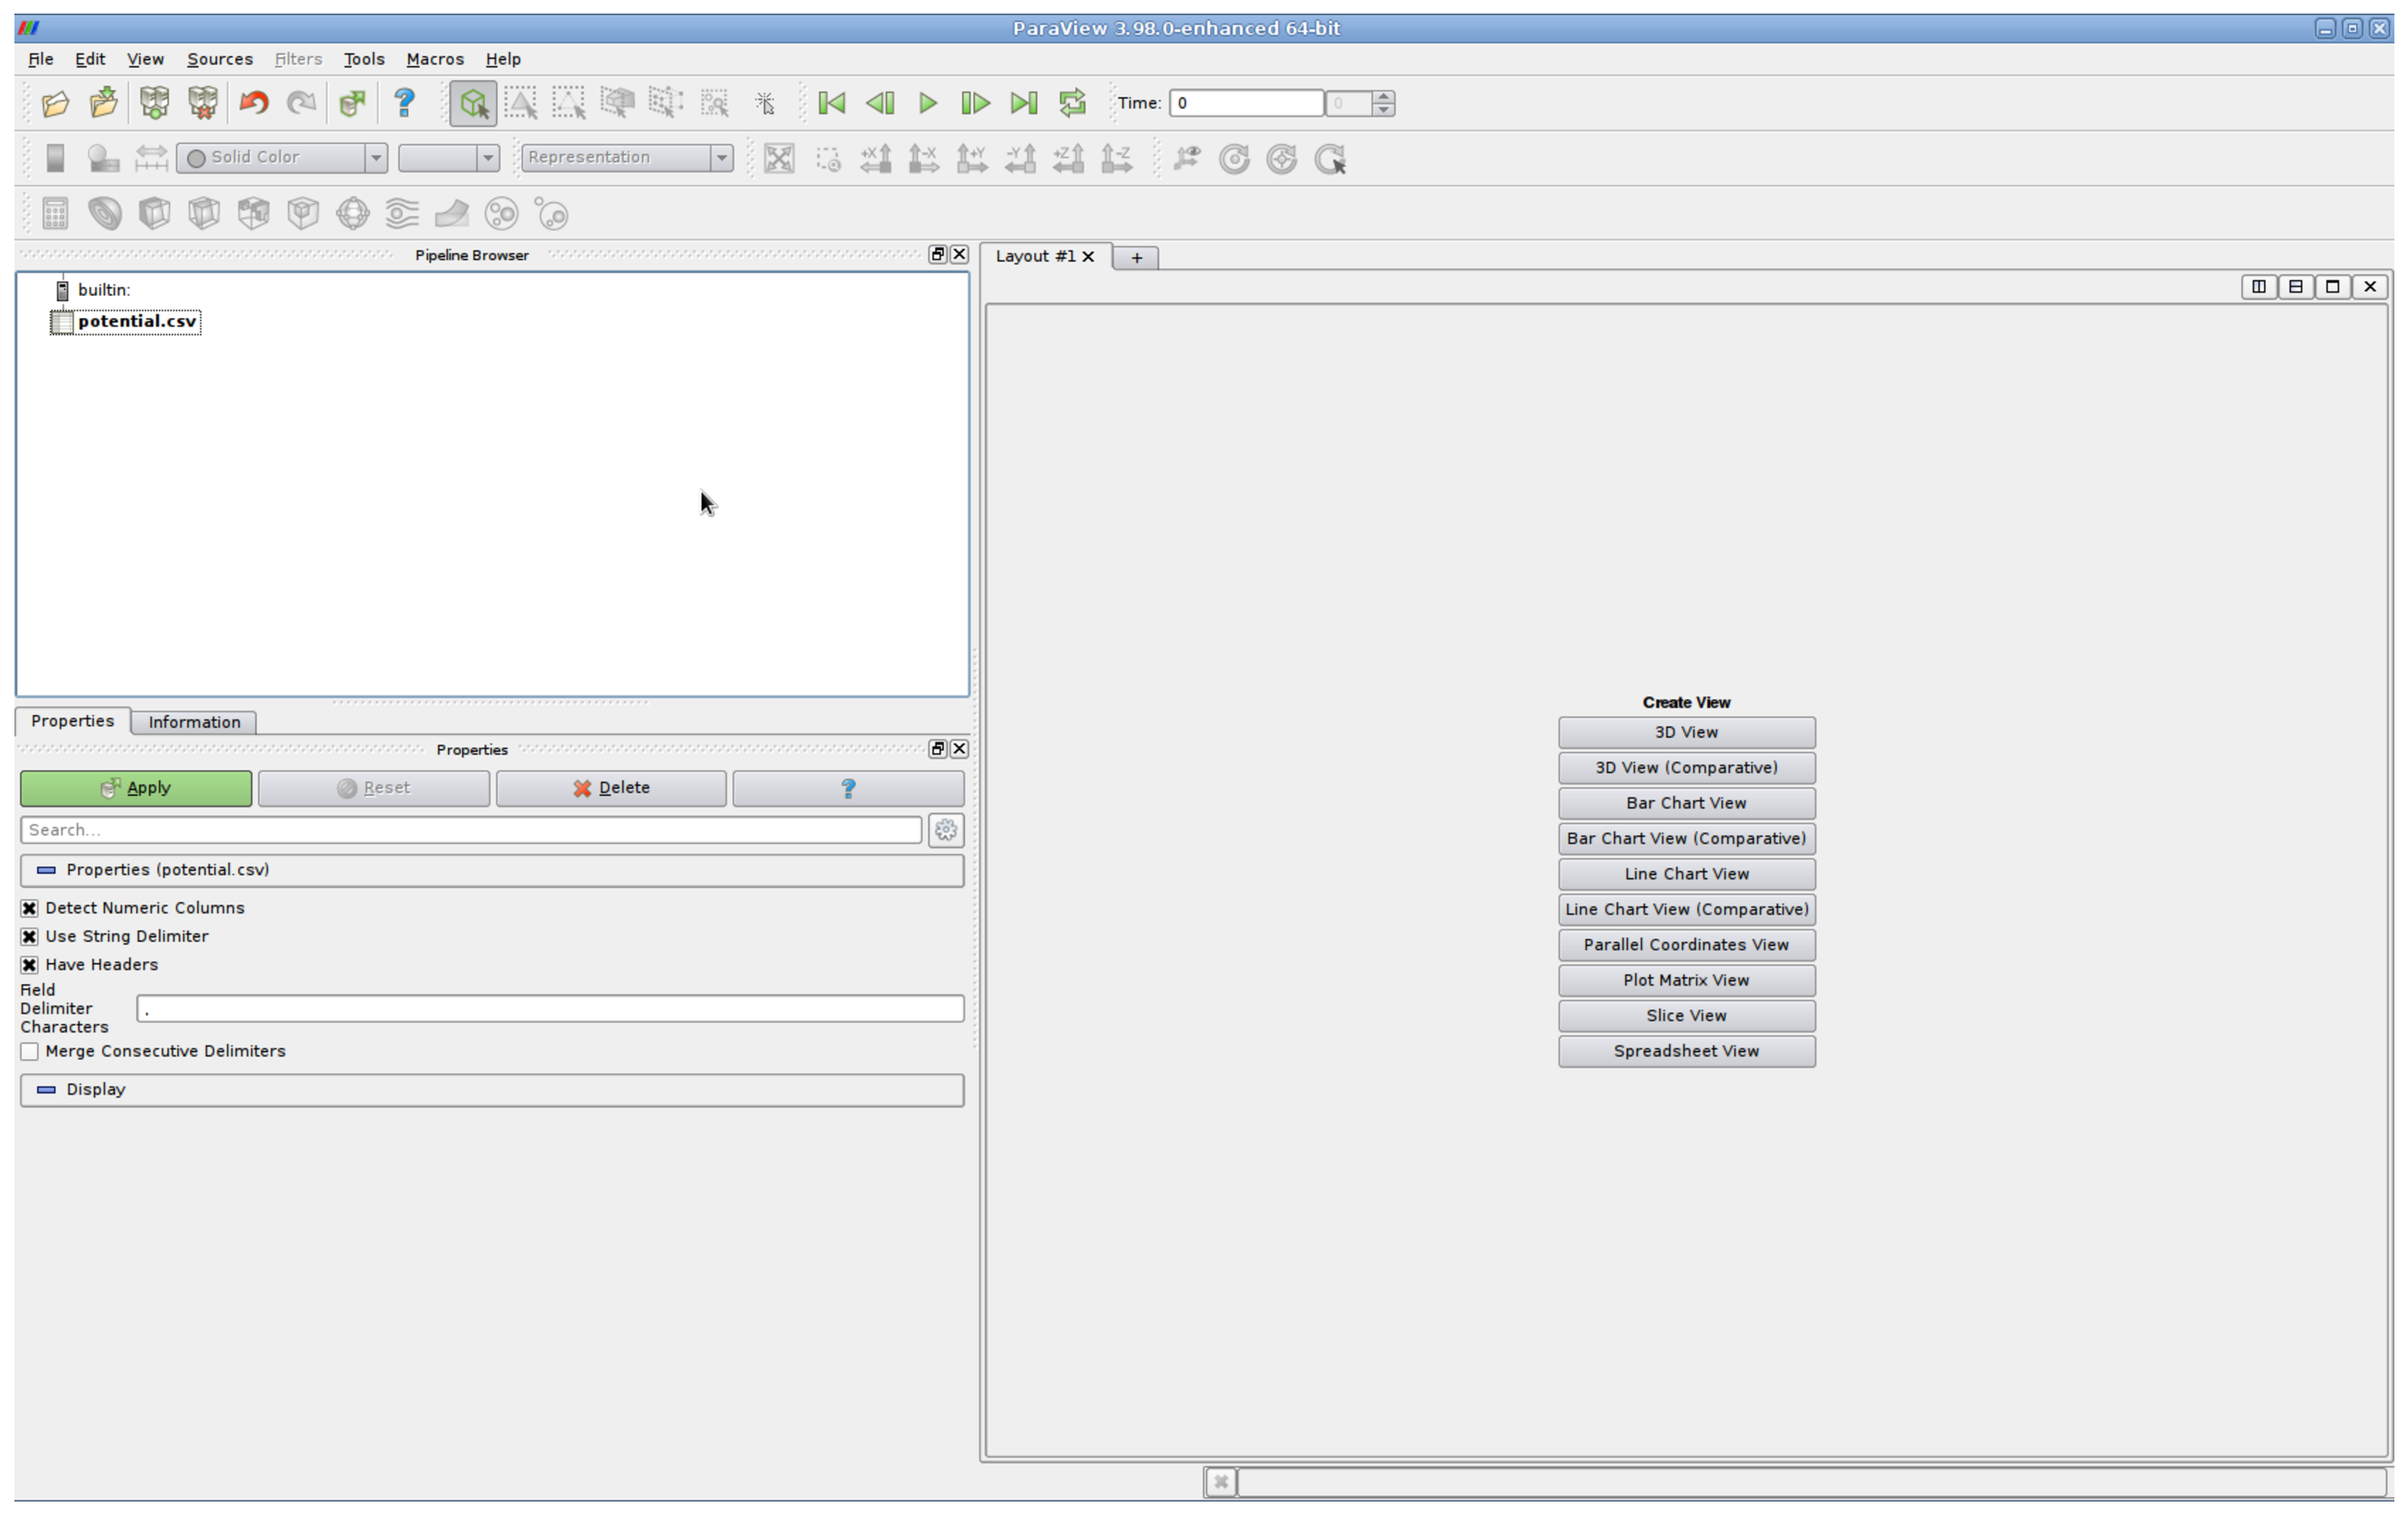
\includegraphics[width=1.0\columnwidth]{figures/para1.eps}
\caption{A CSV file has been loaded into ParaView.}
\label{fig:para1}
\end{figure}


\begin{figure}[!ht]
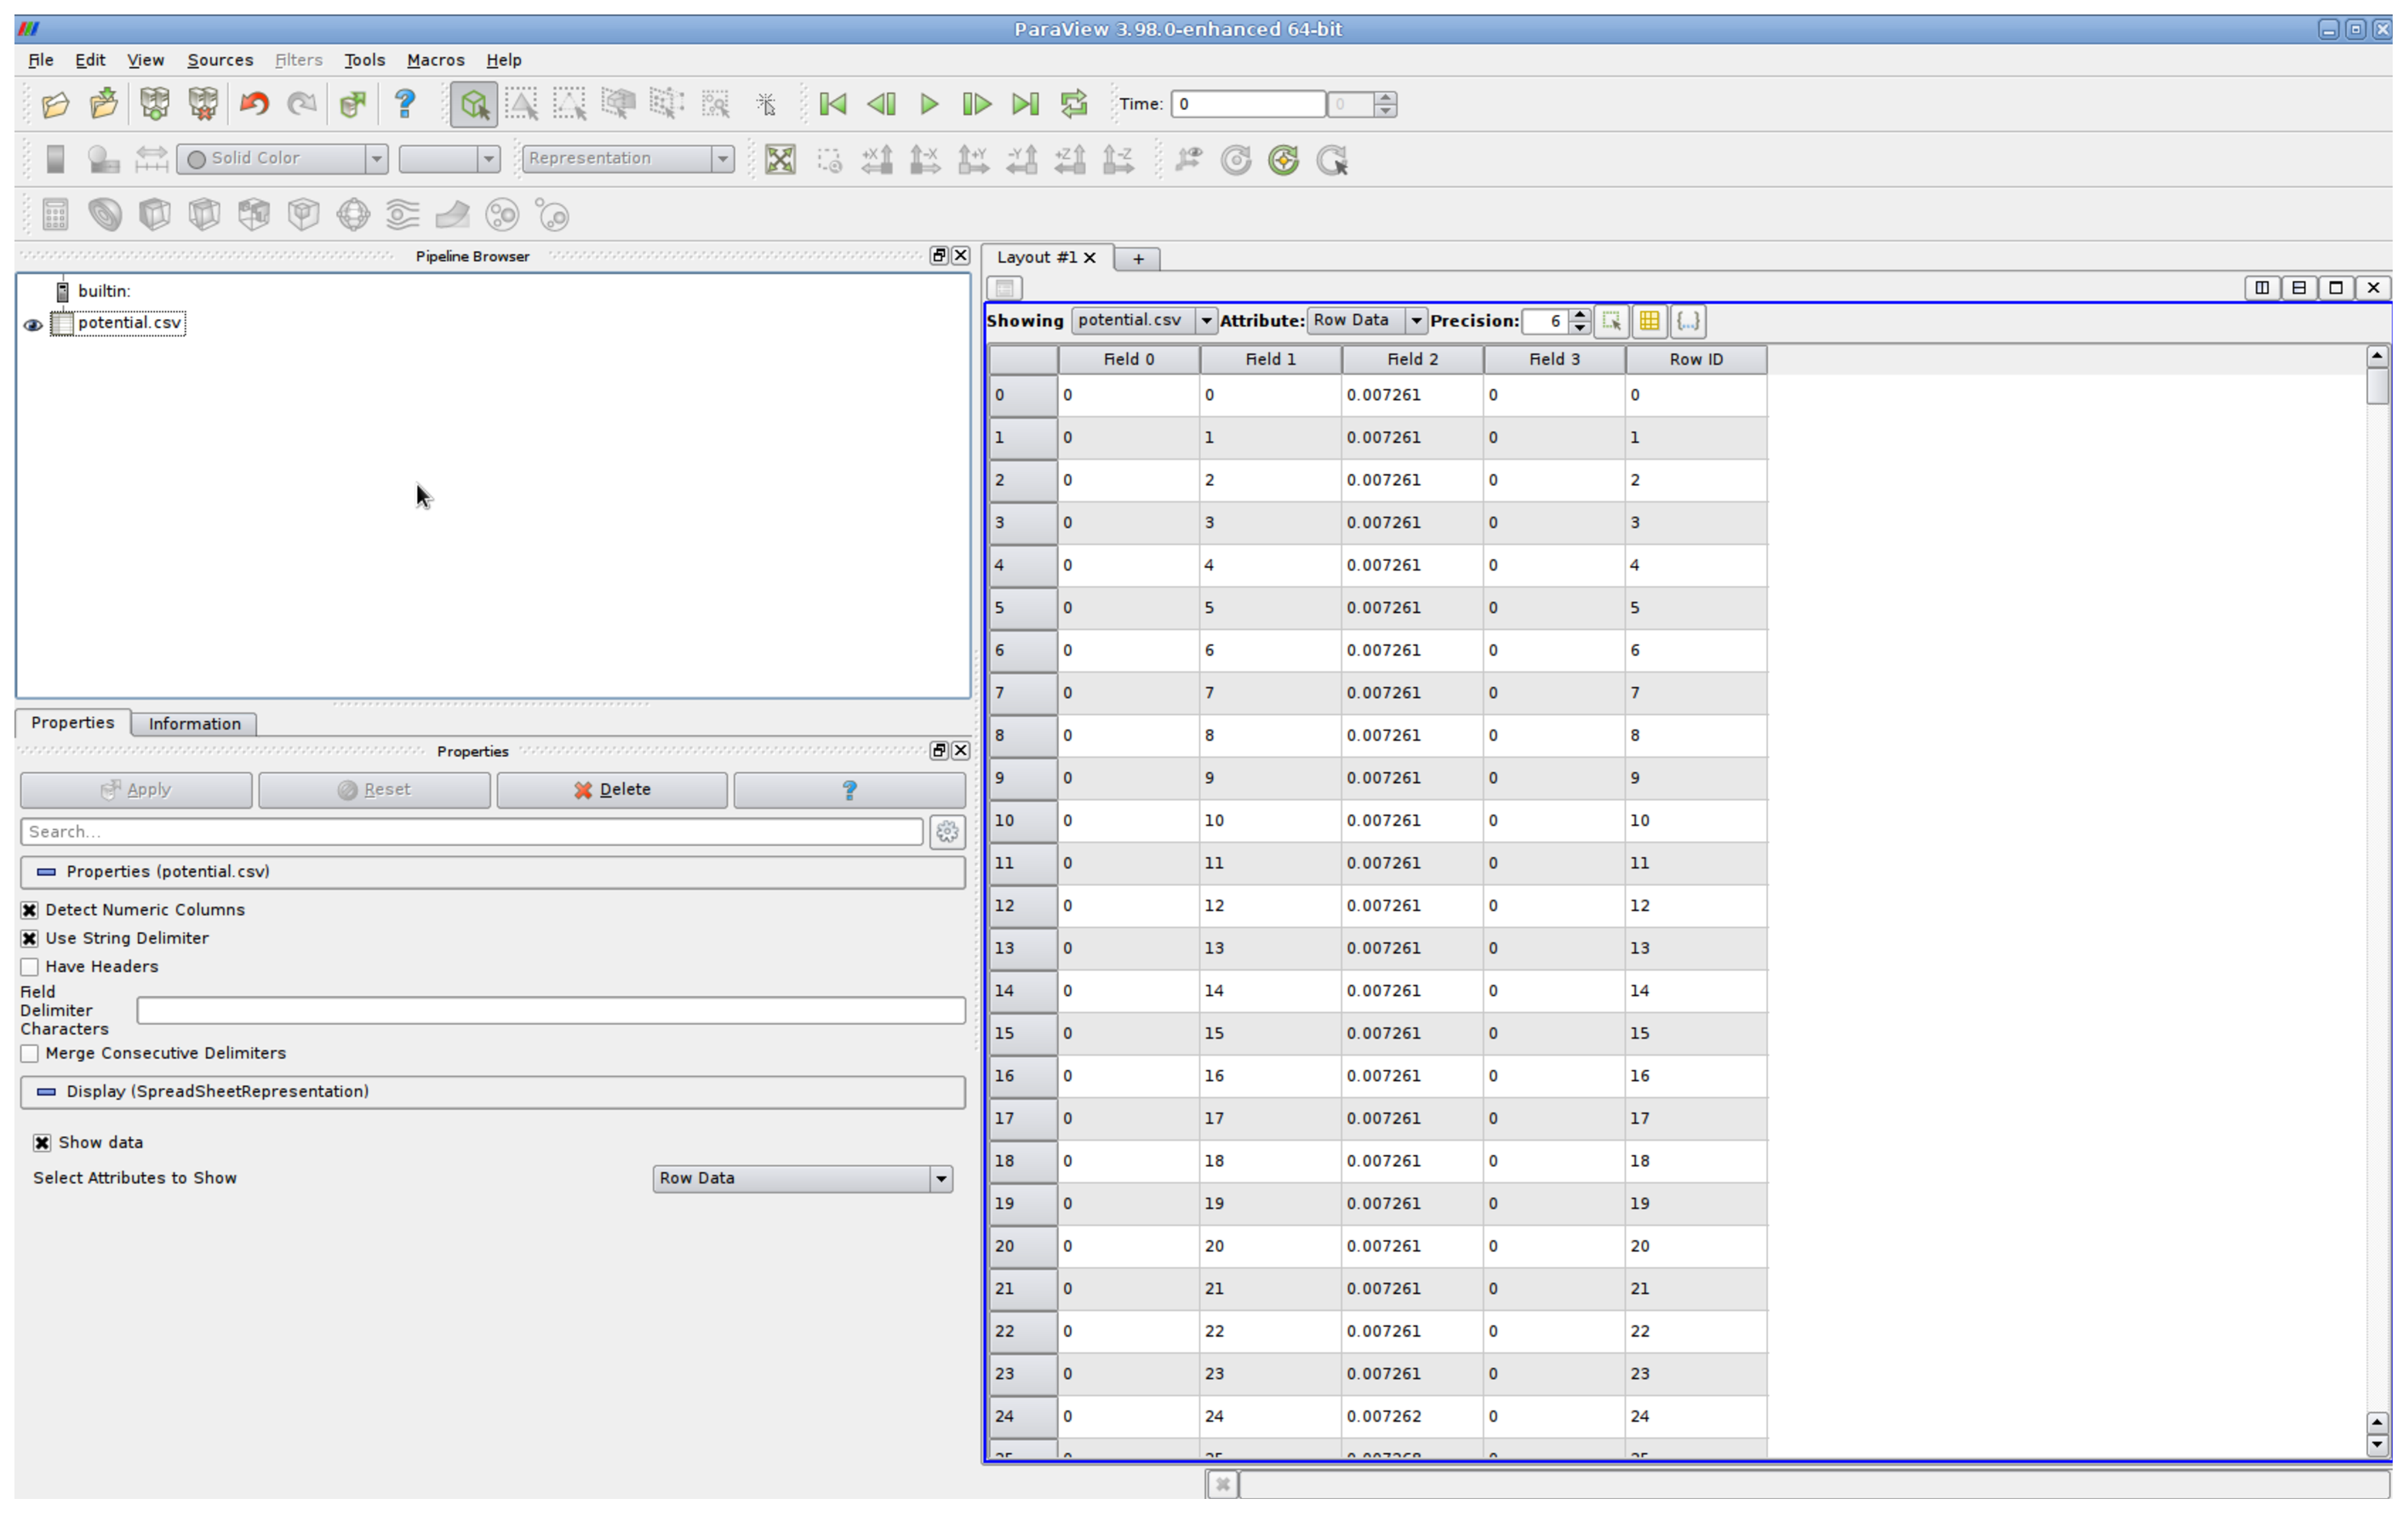
\includegraphics[width=0.9\columnwidth]{figures/para2.eps}
\caption{Headers are deactivated, as well as the comma has been replaced with a whitespace in the delimiter field.
After applying the changes, the table on the right is populated.}
\label{fig:para2}
\end{figure}

\begin{figure}[!ht]
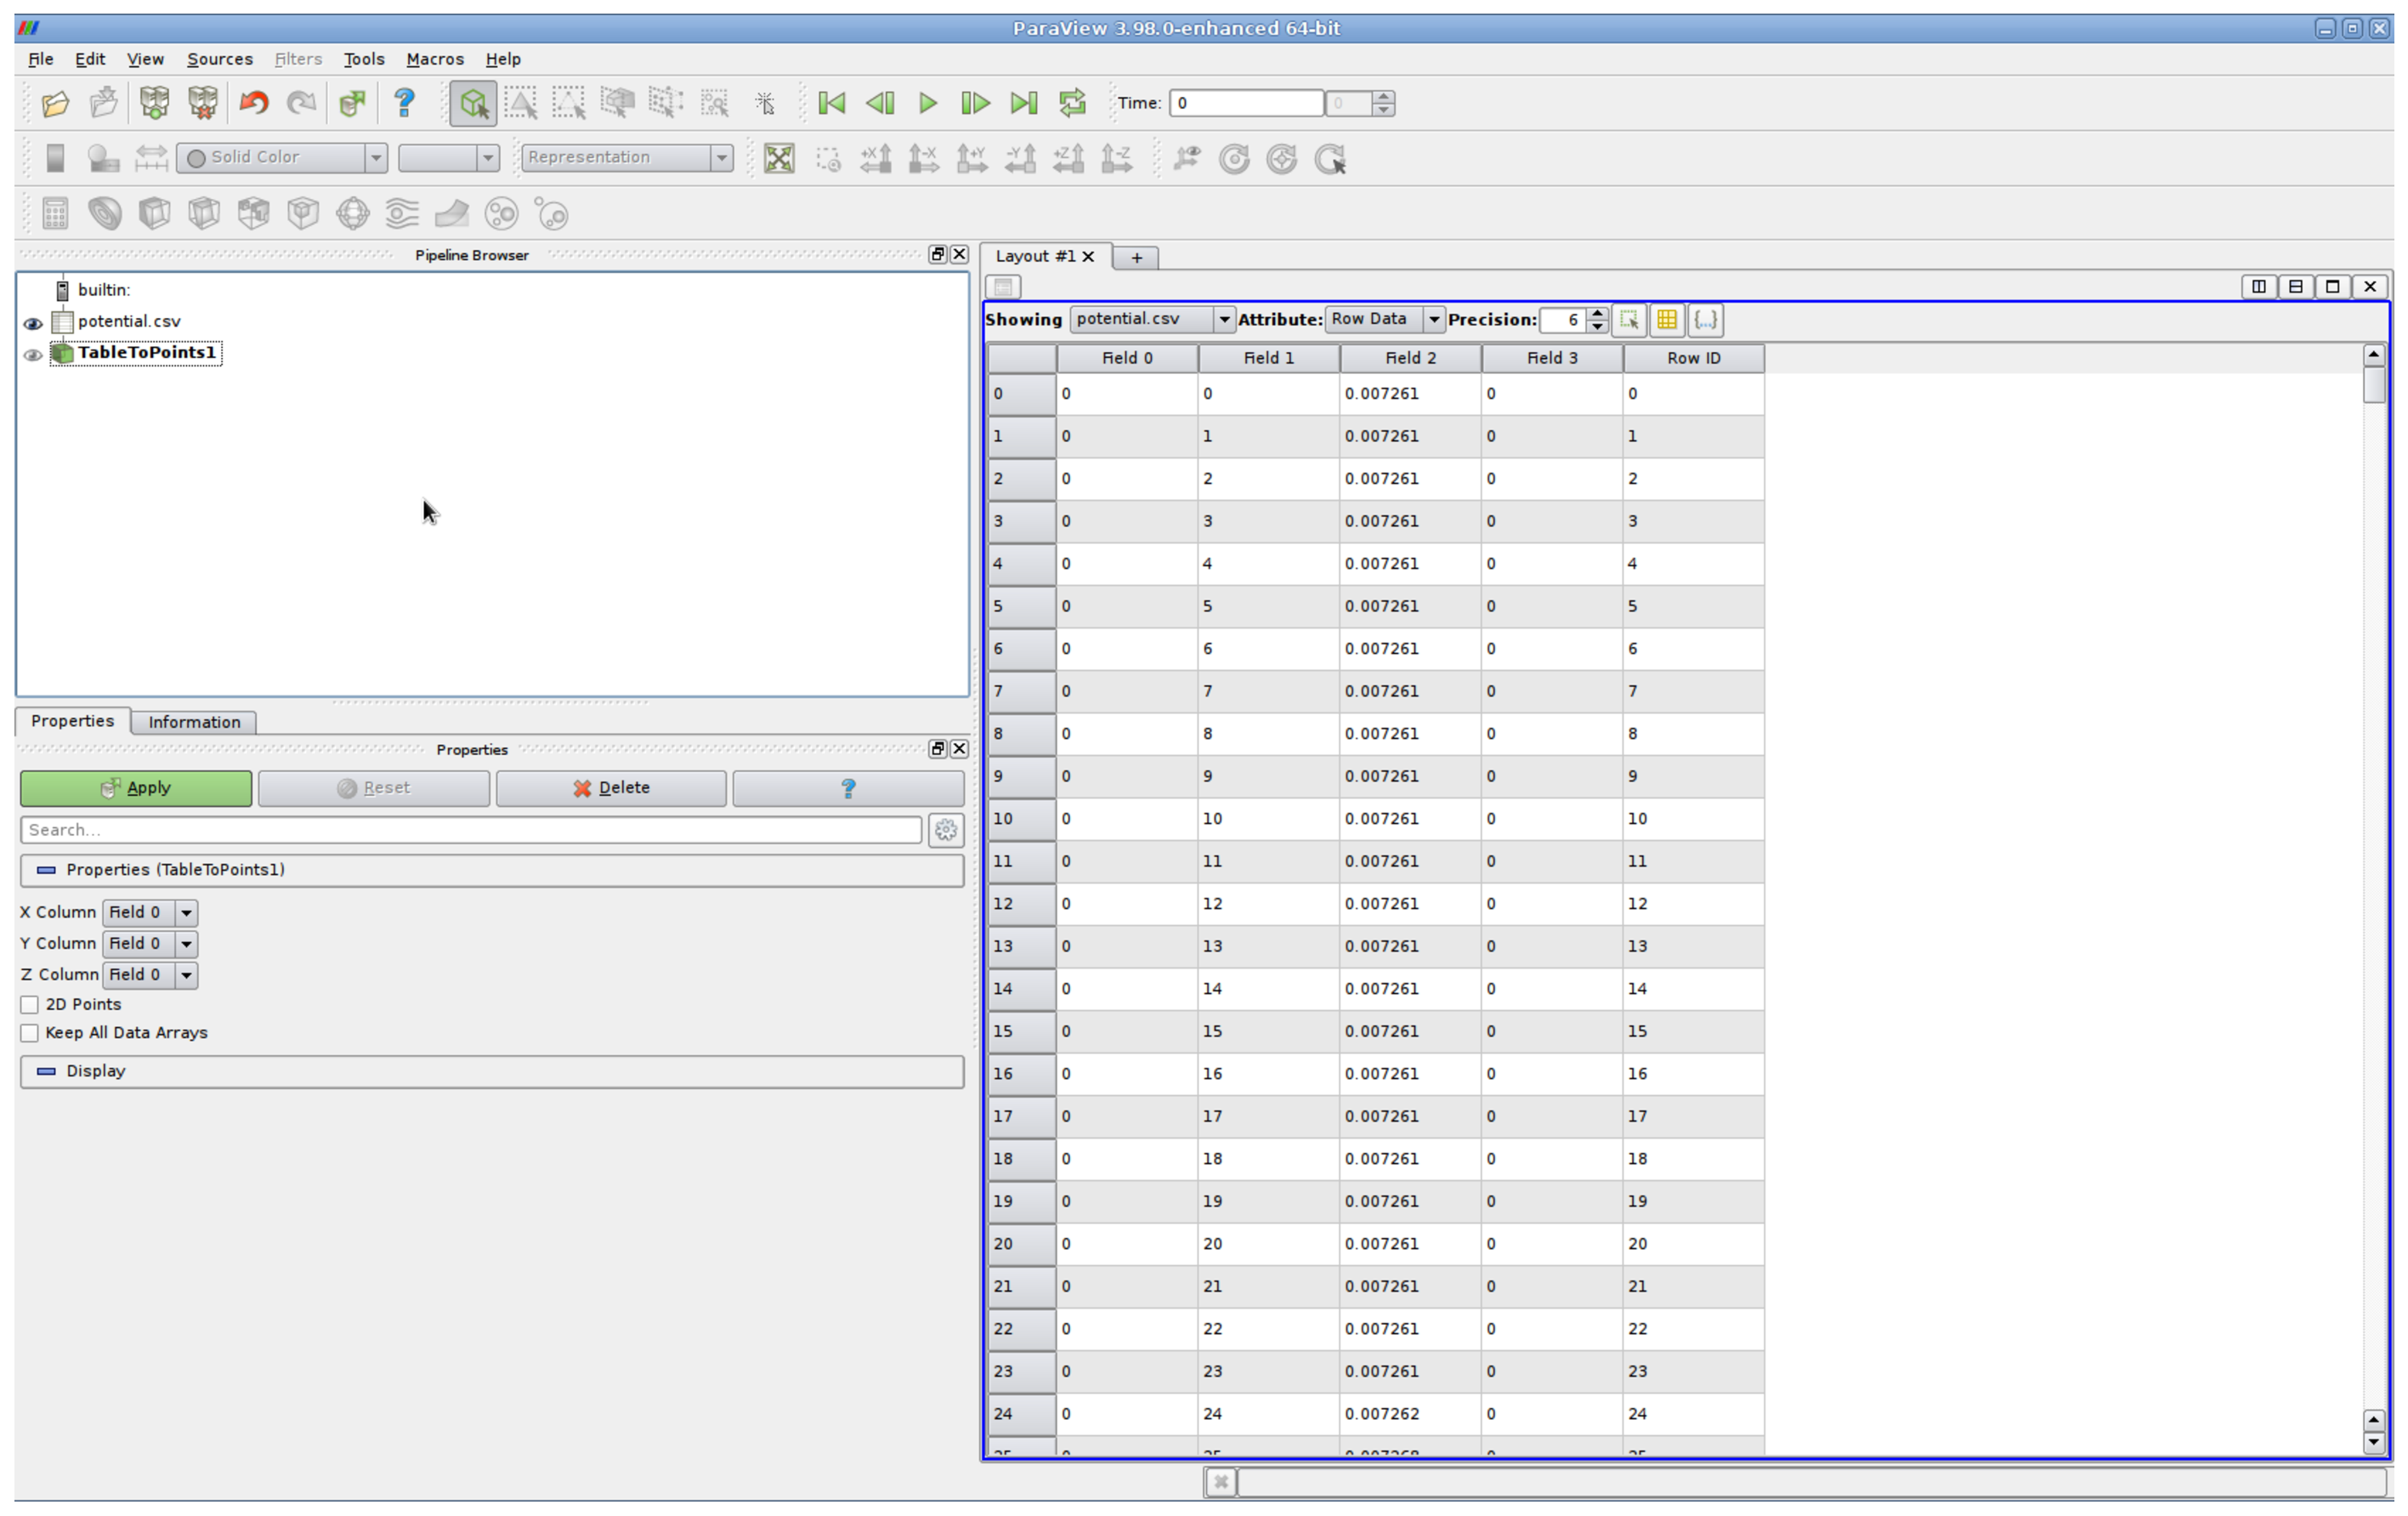
\includegraphics[width=0.9\columnwidth]{figures/para3.eps}
\caption{The \texttt{TableToPoints} filter has been added loaded.}
\label{fig:para3}
\end{figure}

\begin{figure}[!ht]
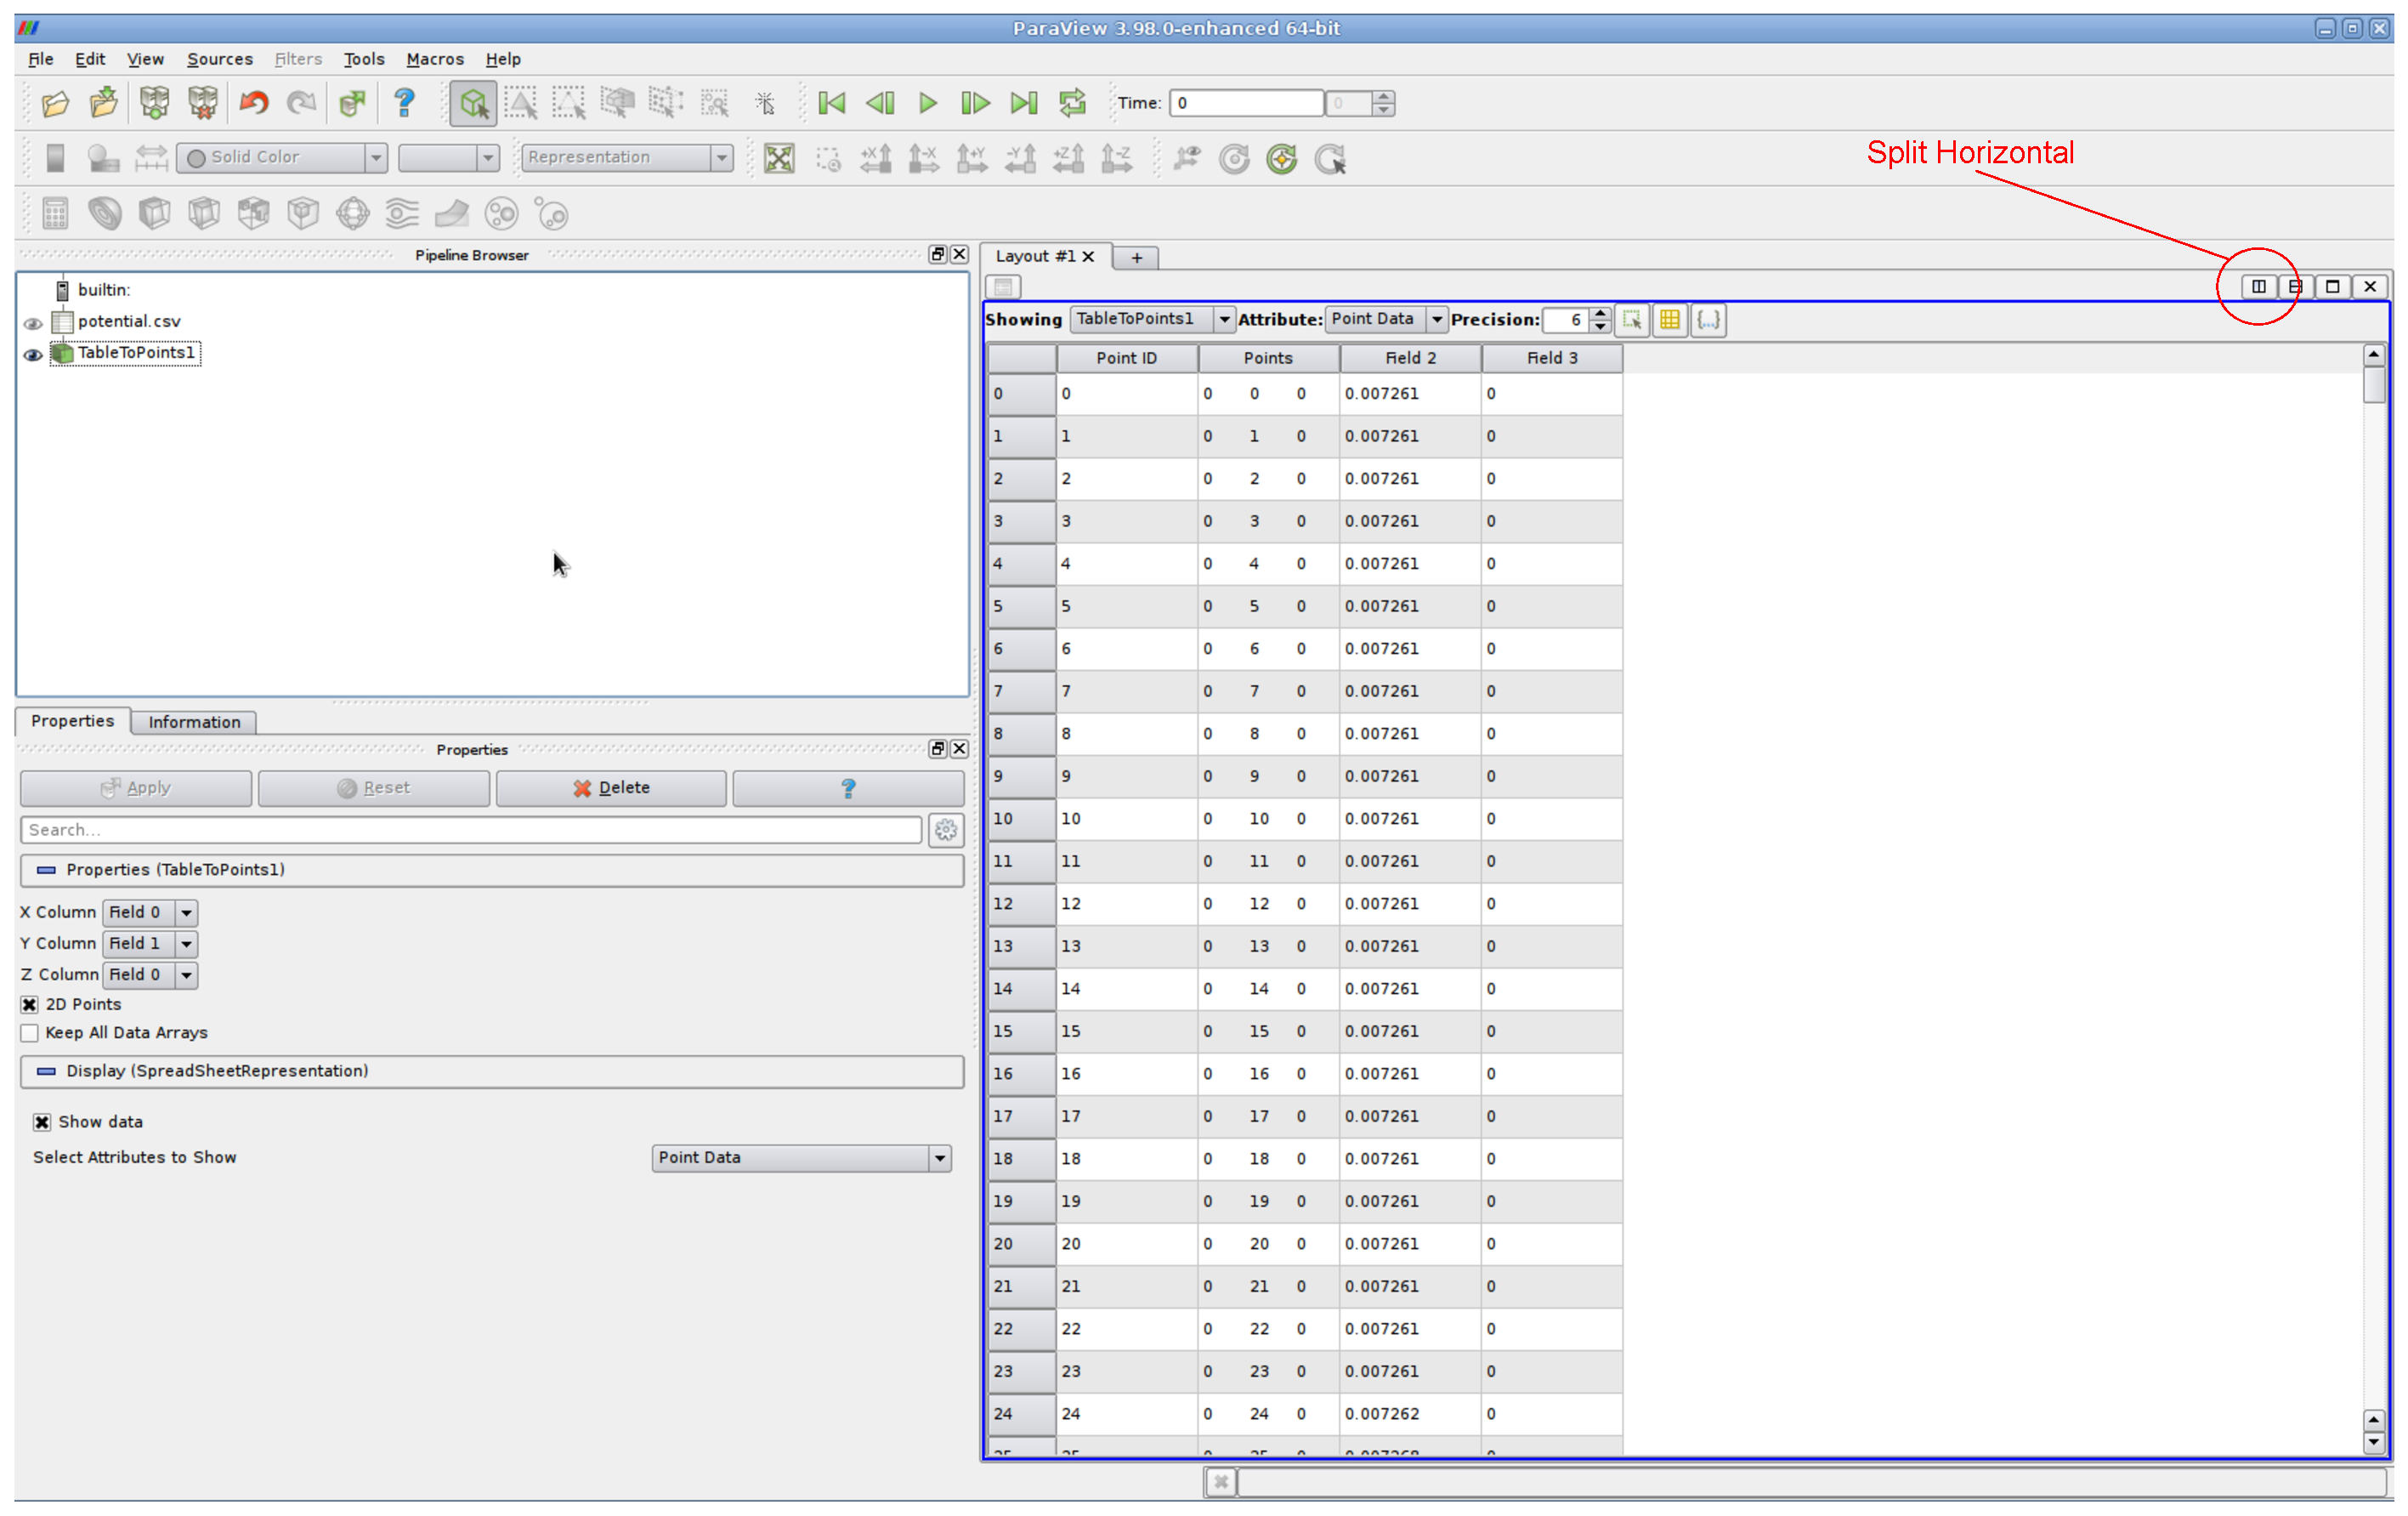
\includegraphics[width=0.9\columnwidth]{figures/para4.eps}
\caption{
The \texttt{TableToPoints} filter has been configured and applied.
Note that the X and Y column has been set to field 0 and 1, respectively.
Furthermore, the table is set to represent 2D data. Note that the Z column is therefore
obsolete.
A new 3D render view has to be created for visualizing the data in the subsequent steps.
This can be achieved, by pushing the \texttt{Split Horizontal} button.
}
\label{fig:para4}
\end{figure}

\begin{figure}[!ht]
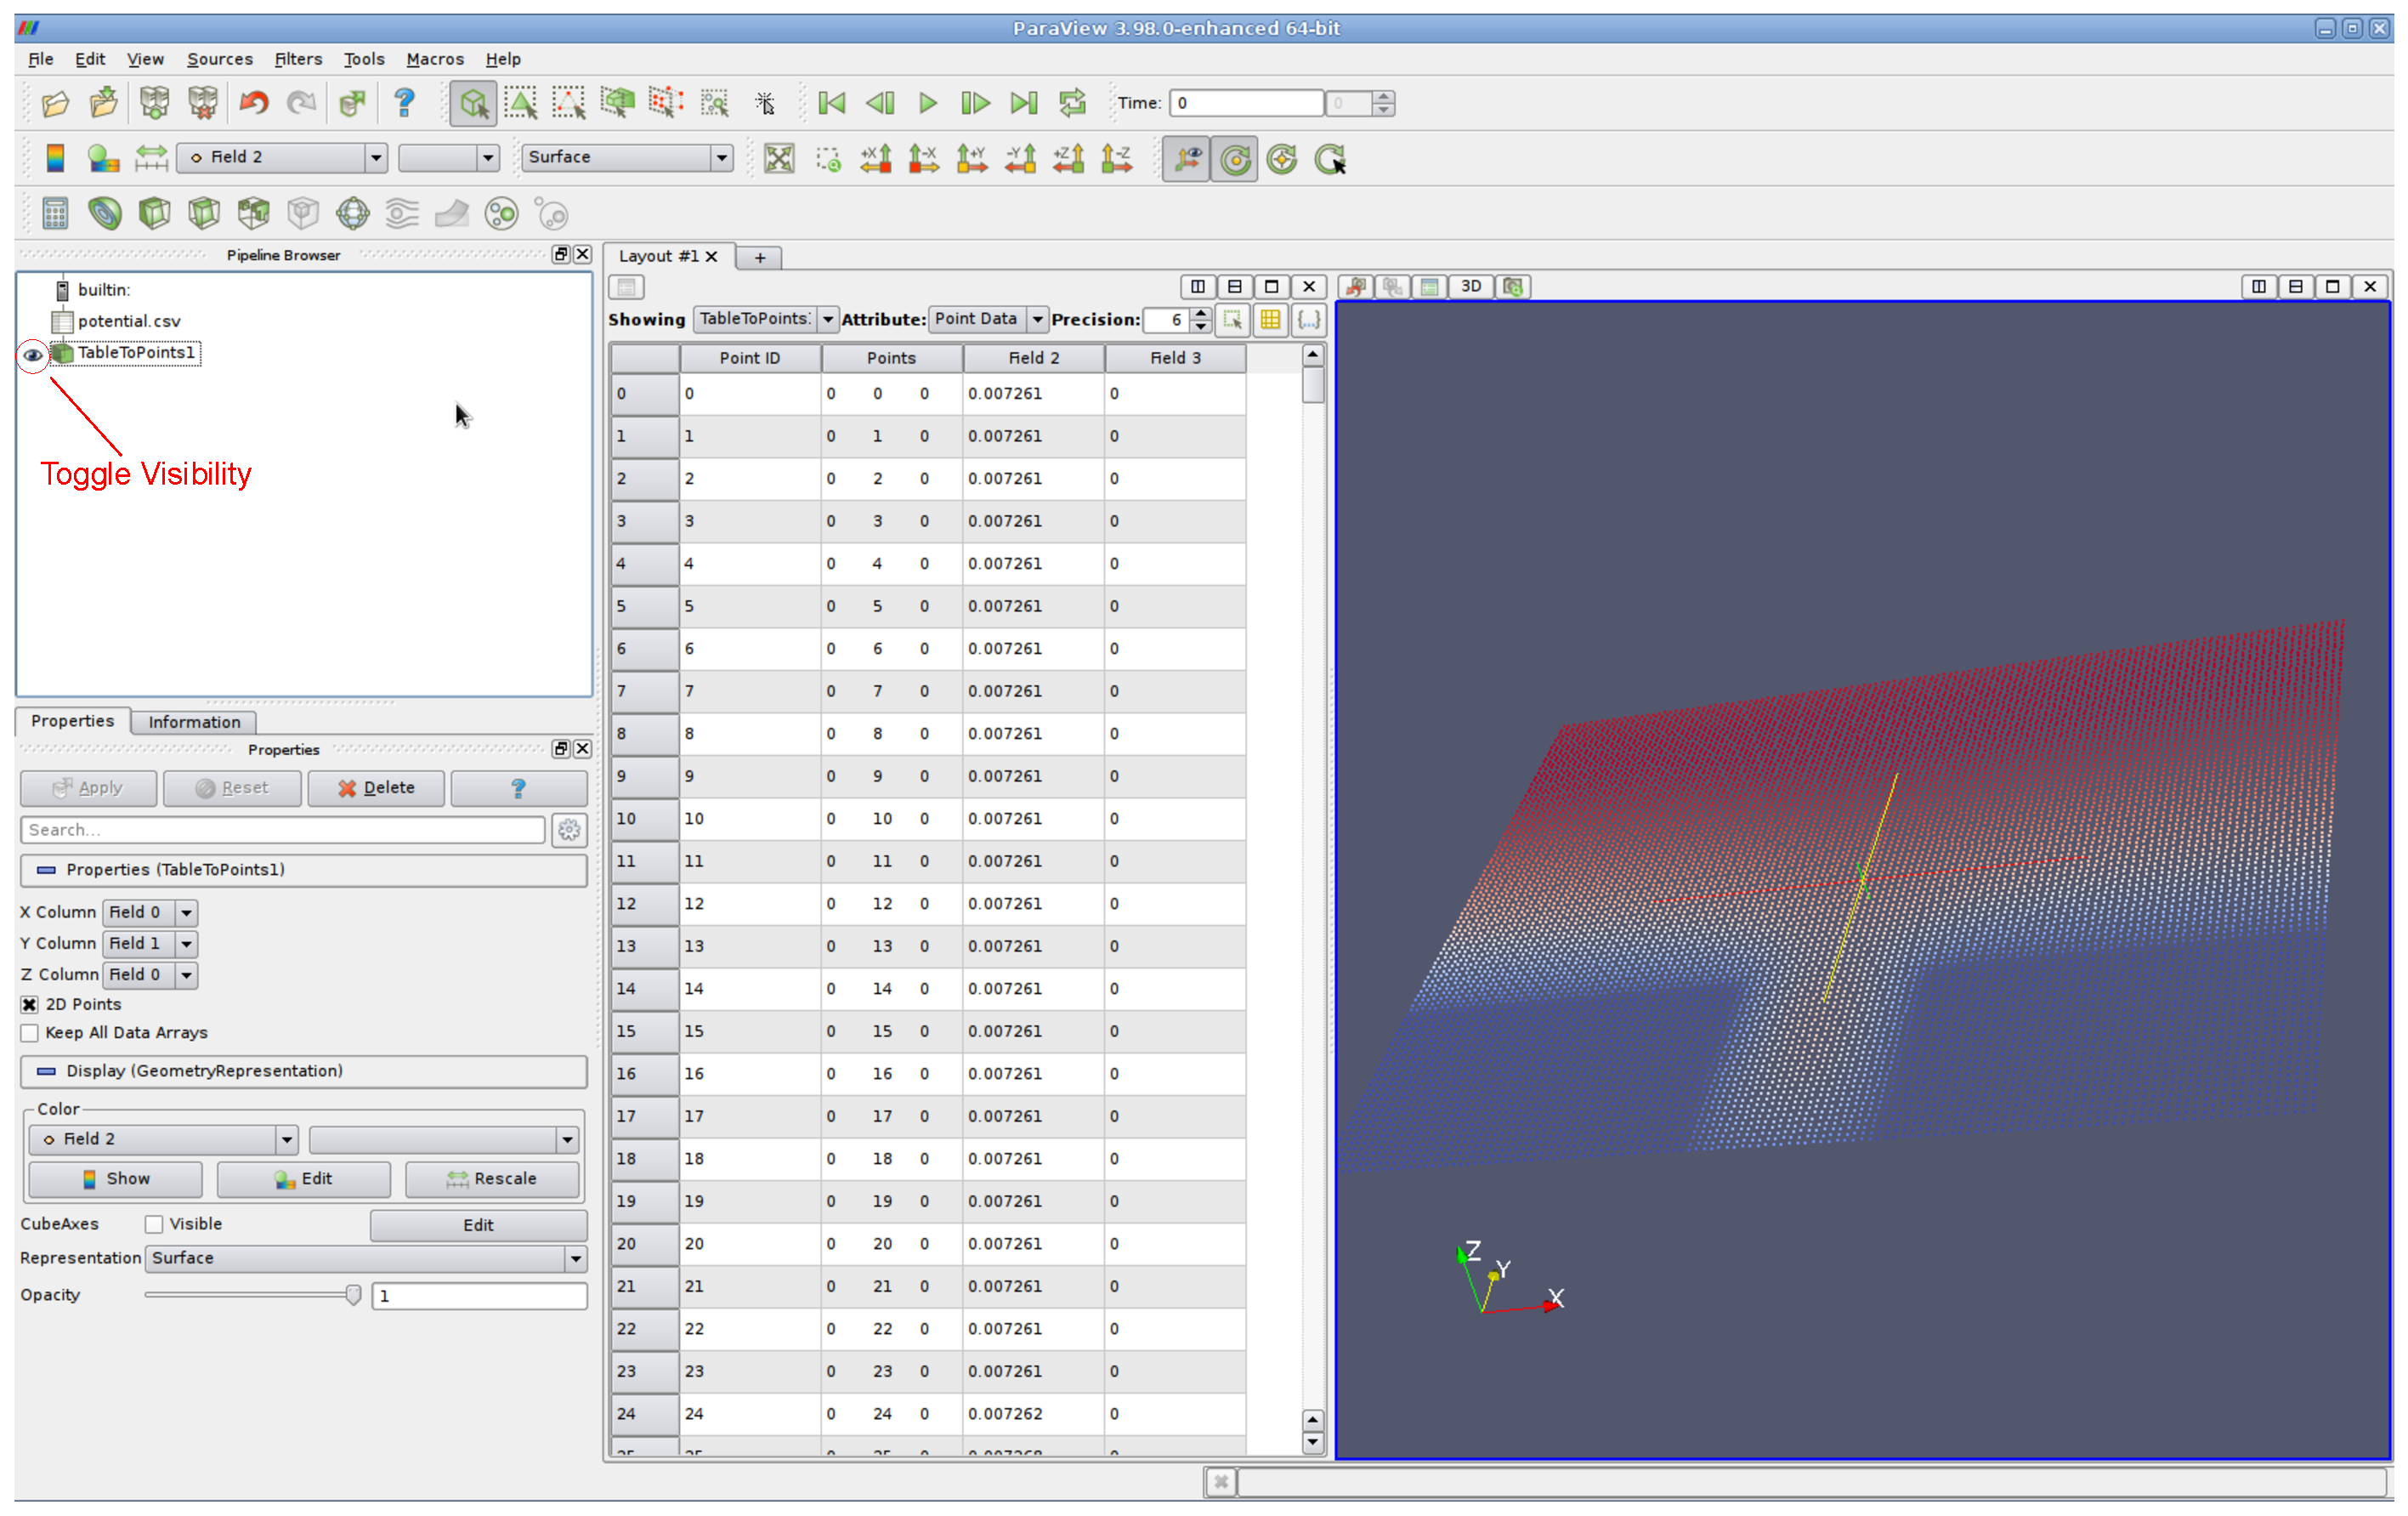
\includegraphics[width=0.9\columnwidth]{figures/para5.eps}
\caption{
The data can be actually visualized by activating the data via
hitting the 'greyed out eye' next to the \texttt{TableToPoints} filter on the left.
Coloring the output can be done by changeing from solid color to a data field, for instance, \texttt{Field 2}.
}
\label{fig:para5}
\end{figure}

\begin{figure}[!ht]
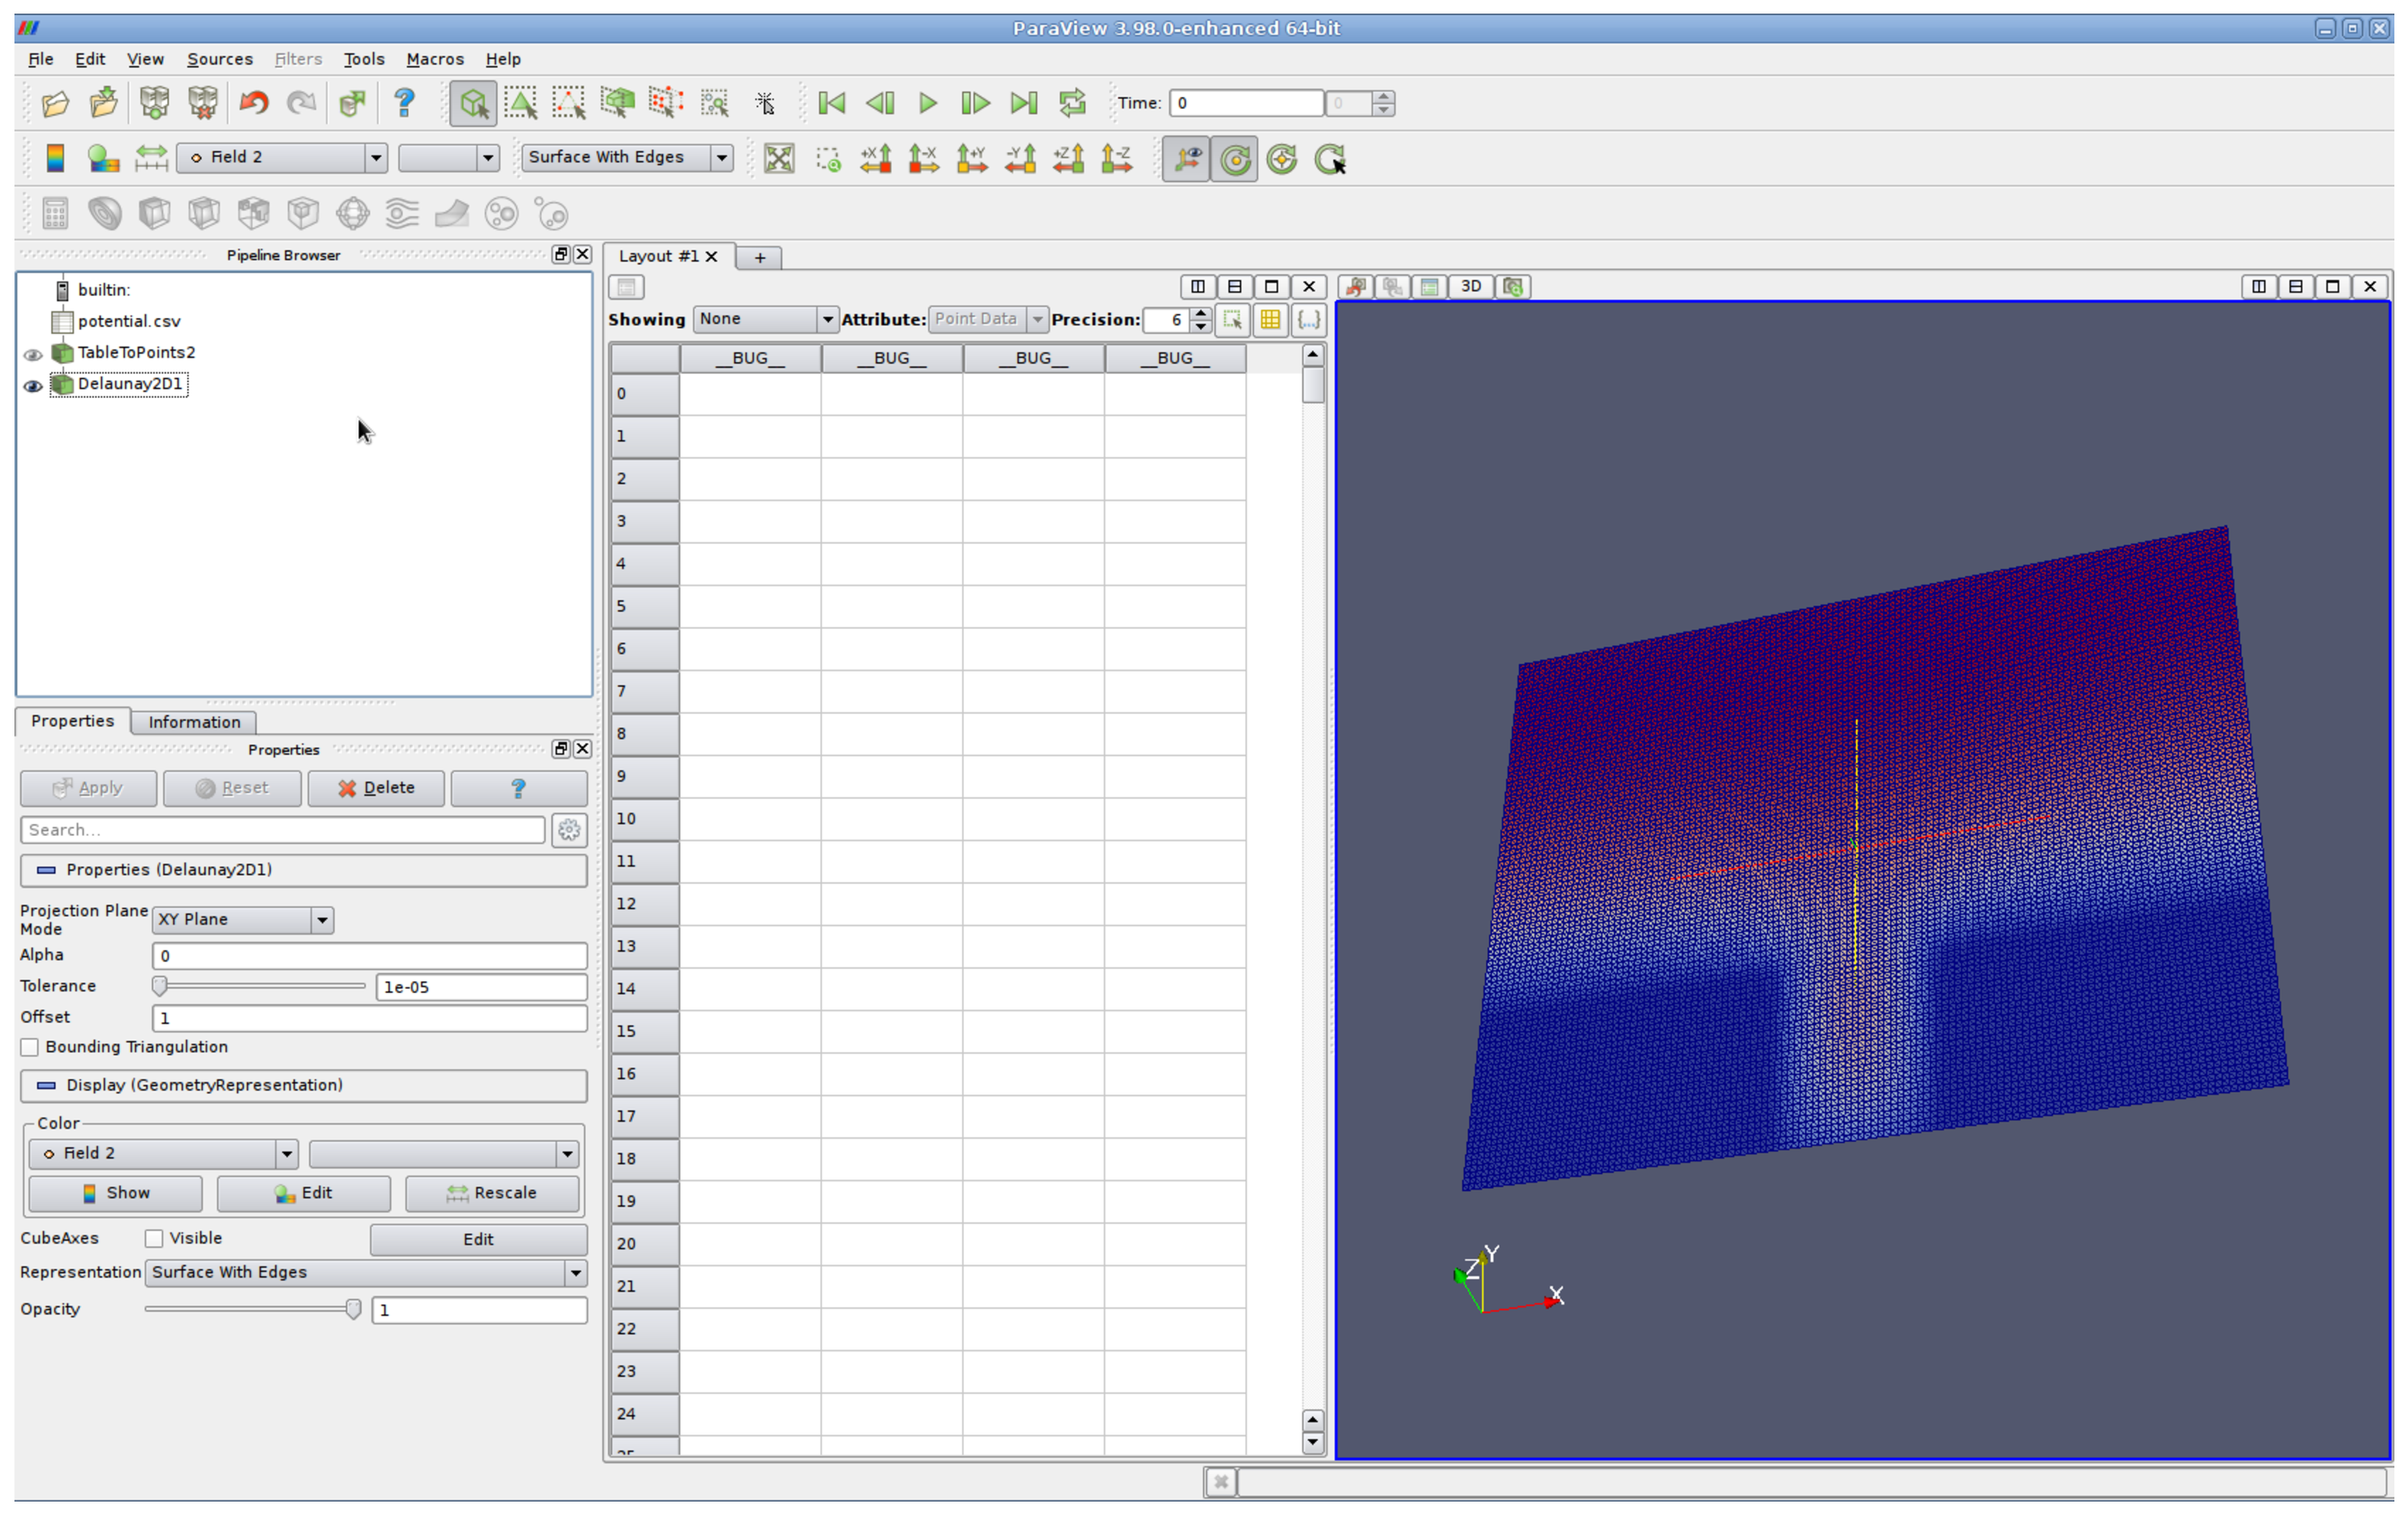
\includegraphics[width=0.9\columnwidth]{figures/para6.eps}
\caption{
So far only points have been visualized, similar to particles.
In case a mesh is required for visualization, the \texttt{Delaunay2D} filter can be used.
No configurations are required, simply adding and applying produces a 2D mesh.
}
\label{fig:para6}
\end{figure}

\begin{figure}[!ht]
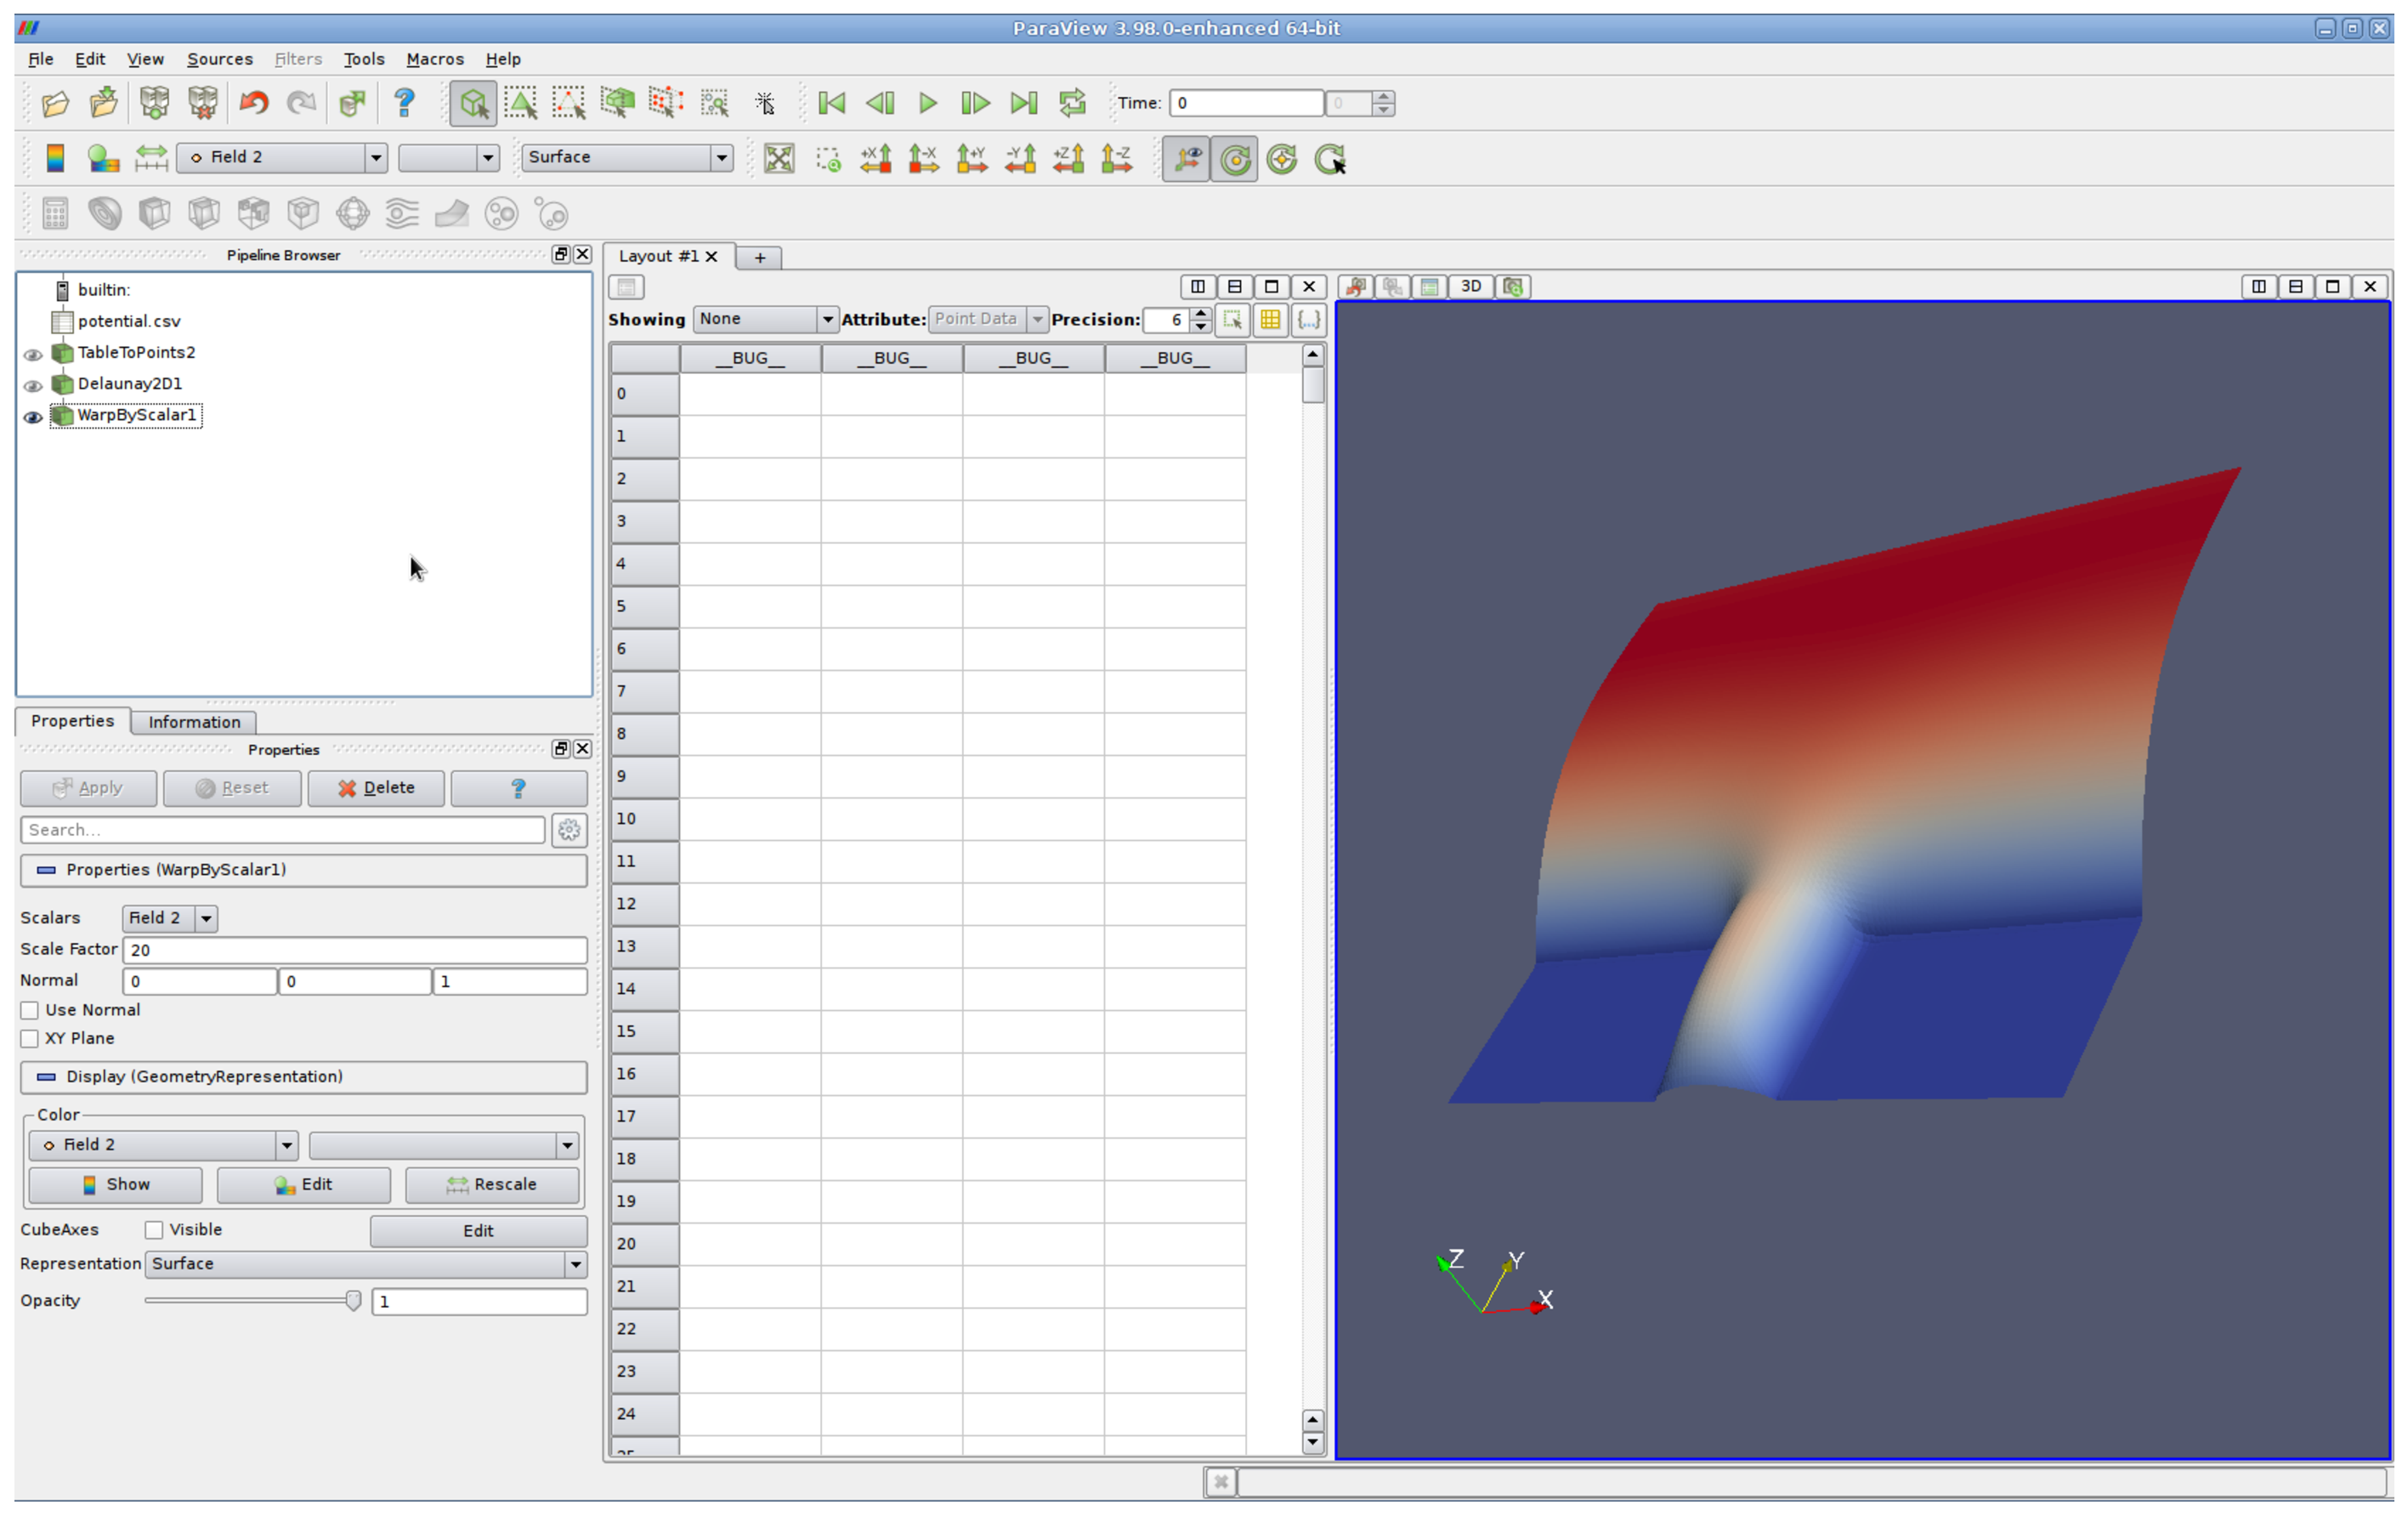
\includegraphics[width=0.9\columnwidth]{figures/para7.eps}
\caption{
For improving the visualization experience of 2D data, the quantity magnitude
can be correlated with a height or Z-coordinate. For this purpose, the \texttt{WarpByScalar} filter can be used.
By changeing the \texttt{Scale Factor} to a higher number, increased scaling is achieved.
}
\label{fig:para7}
\end{figure}
